\section{Computing ADT Complements}
\label{sec:patterns}

TODO MOTIVATE THIS SECTION; ALSO, RETHINK THE TITLE OF THIS SECTION

In addition to the relations $\to_\mathrm{o}$, $\to_\mathrm{p}$, and
$\to_\mathrm{c}$ of Section~\ref{sec:histories} under which all ADTs are
closed, the ADTs we consider in this work are also closed under additional
relations which remove matches, and duplicate operations. The relations
$\to_\mathrm{m}$ and $\to_\mathrm{d}$ relate two histories $h_1$ and $h_2$ when
$h_2$ is obtained from $h_1$ by
\begin{itemize}

  \item removing a match (m), or

  \item removing a duplicate operation (d).

\end{itemize}
We say an ADT closed under $\to_\mathrm{m}$ and $\to_\mathrm{d}$ is
\emph{normal}. In Section~\ref{sec:nature} we demonstrate that
naturally-occurring ADTs are normal. Defining the relation $\succeq$ as the
reflexive and transitive closure of the above relations,
\begin{align*}
  \succeq = (\to_\mathrm{o} \cup \to_\mathrm{p} \cup \to_\mathrm{c} \cup 
  \to_\mathrm{m} \cup \to_\mathrm{d})^\ast
\end{align*}
closure under $\succeq$ follows immediately.

\begin{lemma}

  Normal ADTs are closed under $\succeq$.

\end{lemma}

TODO MOTIVATE WQO

A \emph{well-quasi-ordering (wqo)} $R$ on a set $X$ is a reflexive, transitive
binary relation on $X$ for which in every infinite sequence $x_0 x_1 \ldots$ of
elements from $X$, there exists indices $i < j$ such that $R(x_i,x_j)$.

\begin{example}

  Consider the infinite history sequence $h_1 h_2 \ldots$ where each $h_i$
  contains $2i$ operations $o_1, o_1', \ldots, o_i, o_i'$ where each $o_j$ is a
  completed {\tt push} operation matching itself, and each $o_j'$ is a pending
  {\tt pop} operation with undefined matching. Because each successive $h_i$
  has both more matches and more pending operations, no two histories of the
  sequence are related by $\preceq$. Thus $\preceq$ is not a wqo.

\end{example}

The previous example demonstrates that $\preceq$ is not a wqo by allowing each
history $h_i$ of the infinite sequence to contain more and more pending
operations in order to ensure that $h_j \not\preceq h_i$ for every $j < i$.
Curbing this ability by limiting the maximum amount of pending operations per
history makes $\preceq$ a wqo. Although limiting to $k$ pending operations
essentially limits us to width-$k$ histories, of executions with at most $k$
operations parallel at any moment, e.g.,~of programs with at most $k$ threads,
this restriction comes at no loss of completeness when considering only the
histories of bounded-width ADT kernels, which is the subject of the remainder
of this section.

\begin{lemma}

  $\preceq$ is a wqo on width-bounded histories.

\end{lemma}

For the remainder of this section, we fix an ADT $A$, and let $B$ be the
complement of $\ker A$. When $\ker A$ has bounded width, so does $B$, and thus
$\preceq$ is a wqo on $B$. Furthermore, when $A$ normal, it is closed under
$\succeq$, and thus $B$ is closed under $\preceq$. Closure under a wqo implies
representation by a finite set. Formally, we say a set $X$ is \emph{finitely
representable} if there exists a finite set $Y$ and a relation $R \subseteq Y
\times X$ such that $X = \set{ x : \exists y\in Y.\ R(y,x) }$. In our case, we
obtain a finite set from which exactly the elements of $B$ are related by
$\preceq$.

\begin{lemma}

  $B$ is finitely representable if $A$ is normal.

\end{lemma}

Computing $B$ thus amounts to computing its finite representation. In general,
this is achieved by enumerating the elements of $B$ while maintaining the
$\preceq$-minimal elements, and recognizing a condition under which all
elements of $B$ are related to the current set of
minimals~\cite{conf/lics/AbdullaCJT96, journals/tcs/FinkelS01}. In our case, we
recognize a condition on the weight-increasing enumeration of $B$ which
guarantees coverage by the current set of minimals. Formally, for all $i \in
\mathbb{N}$, we define
\begin{align*}
  B_i &= \set{ h \in B : \weight(h) \le i } \\
  B_i' &= \set{ h' \in B :
    \exists h \in B_i.\ h \preceq h' \text{ and } \weight(h') \le i+1
  }
\end{align*}
as, respectively, the histories of $B$ with at most $i$ matches and duplicates,
and those derived from $B_i$ with at most $i\!+\!1$ matches and duplicates. We
say that $A$ is \emph{predictable} if $B_i = B$ whenever $B_i' = B_{i+1}$. In
Section~\ref{sec:nature} we demonstrate that naturally-occurring ADTs are
predictable. Since the number of weight-$i$ histories is finite\footnote{As
noted in Section~\ref{sec:histories}, we consider equality between histories up
to renaming of operation identifiers.} for each $i \in \mathbb{N}$, each $B_i$
is computable.

\begin{lemma}

  $B_i$ is computable, for all $i \in \mathbb{N}$, if $A$ is normal.

\end{lemma}

Predictability ensures that once $B_{i+1}$ does not alter the set of computed
$\preceq$-minimals, with respect to those of $B_i$, then the minimals computed
for $B_i$ are exactly those of $B$.

\begin{lemma}

  $B$ is computable if $A$ is normal and predictable.

\end{lemma}

Note that for non-predictable ADTs, computing $B_i$, for any $i \in
\mathbb{N}$, under-approximates $B$. In practice, computing $B_i$ can be used
to identify all violations which surface in histories with $i$ matches,
overlooking violations which only surface with more than $i$ matches. The
resulting symbolic ADT representation would still be sound in only identifying
\emph{actual} violations, yet incomplete in identifying \emph{all} violations.

\begin{example}

  TODO EXAMPLE OF COMPLETE PATTERNS

  \begin{figure}[t]
    \centering
    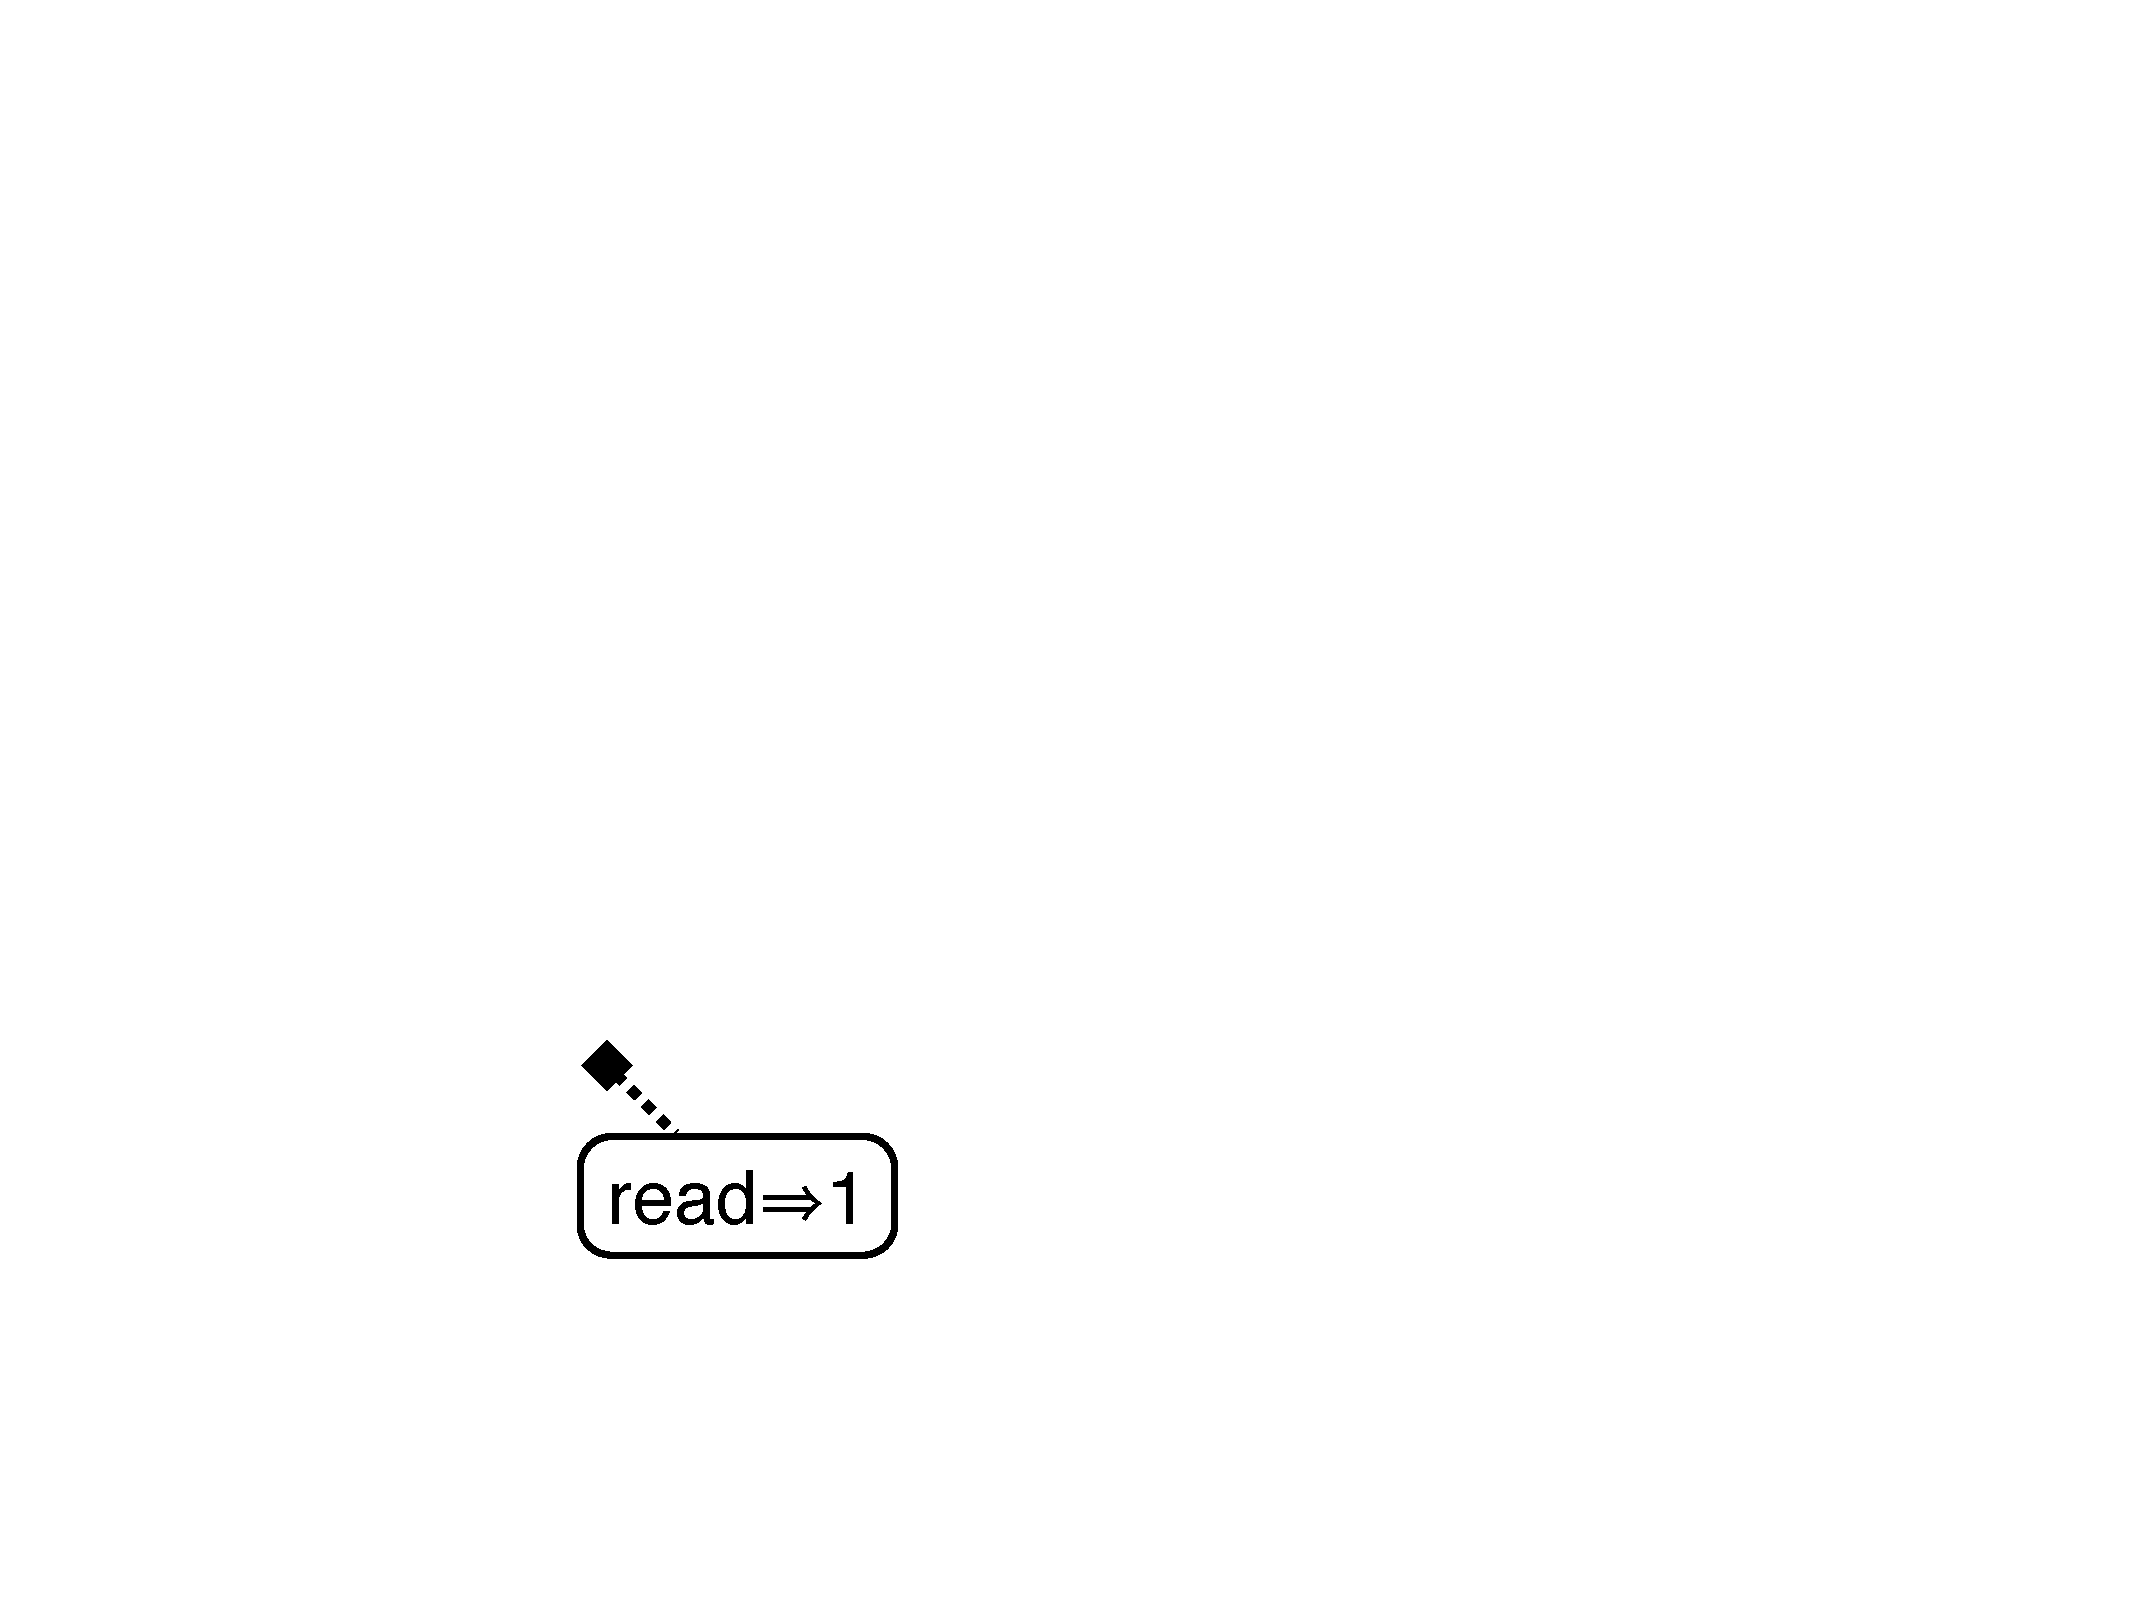
\includegraphics[scale=0.2]{figures/register-pattern-1},
    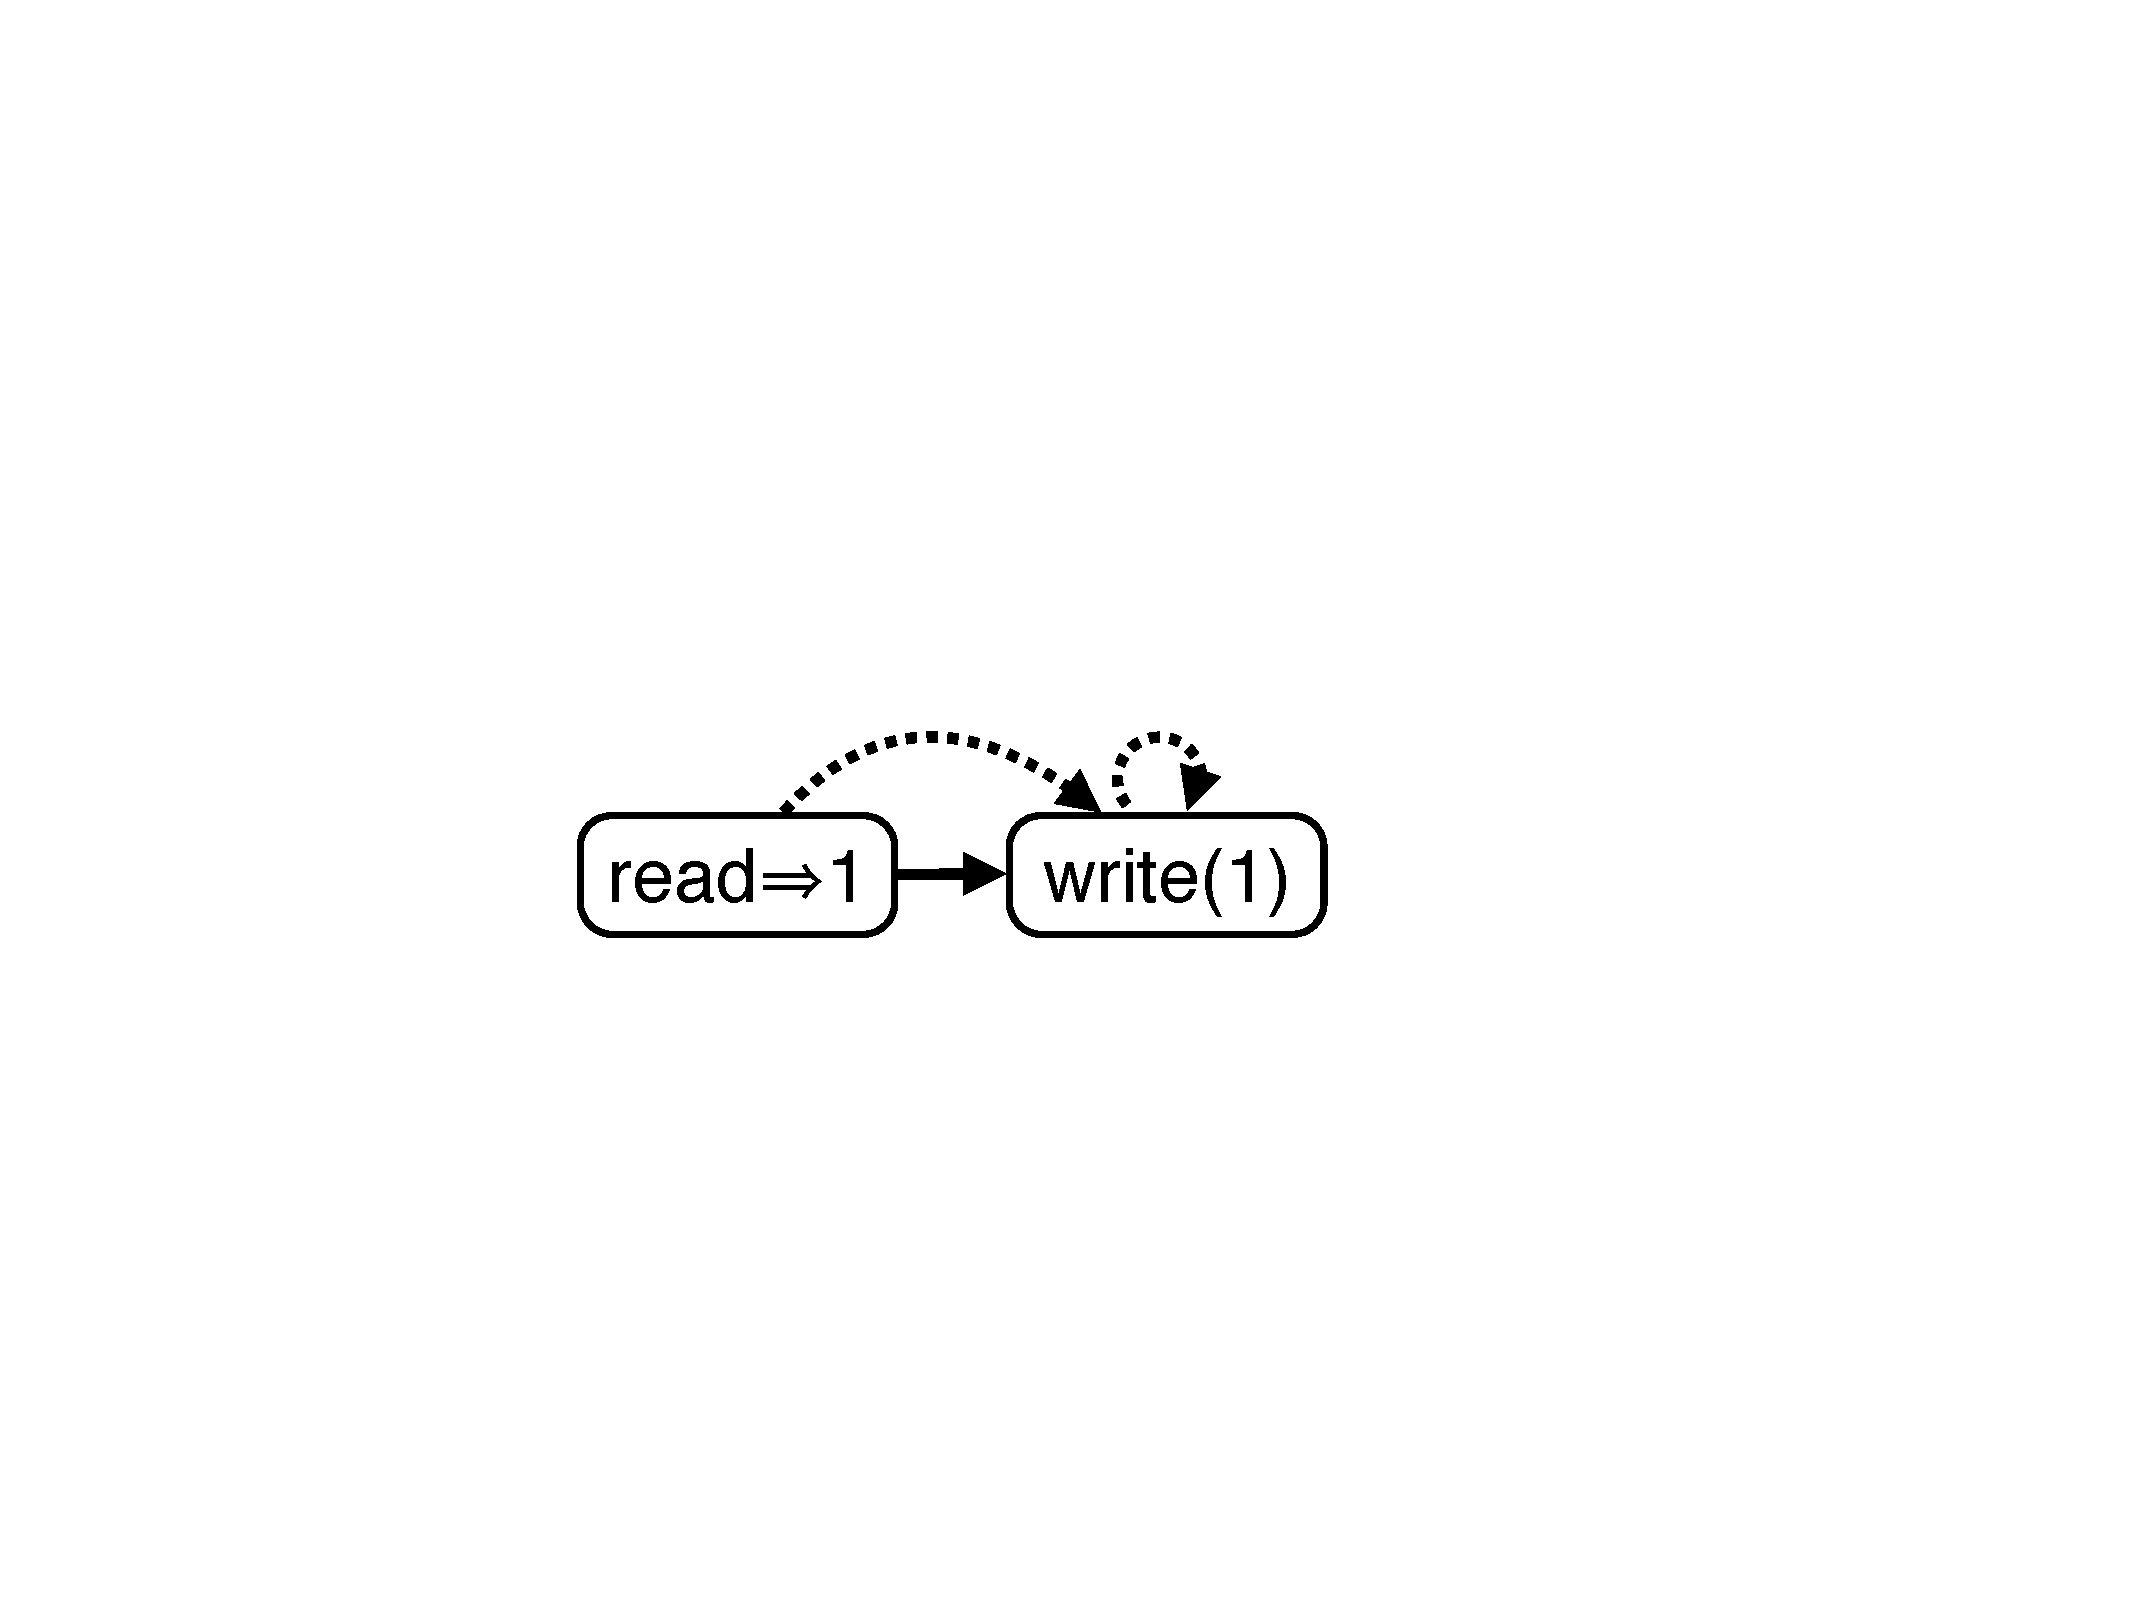
\includegraphics[scale=0.2]{figures/register-pattern-2},
    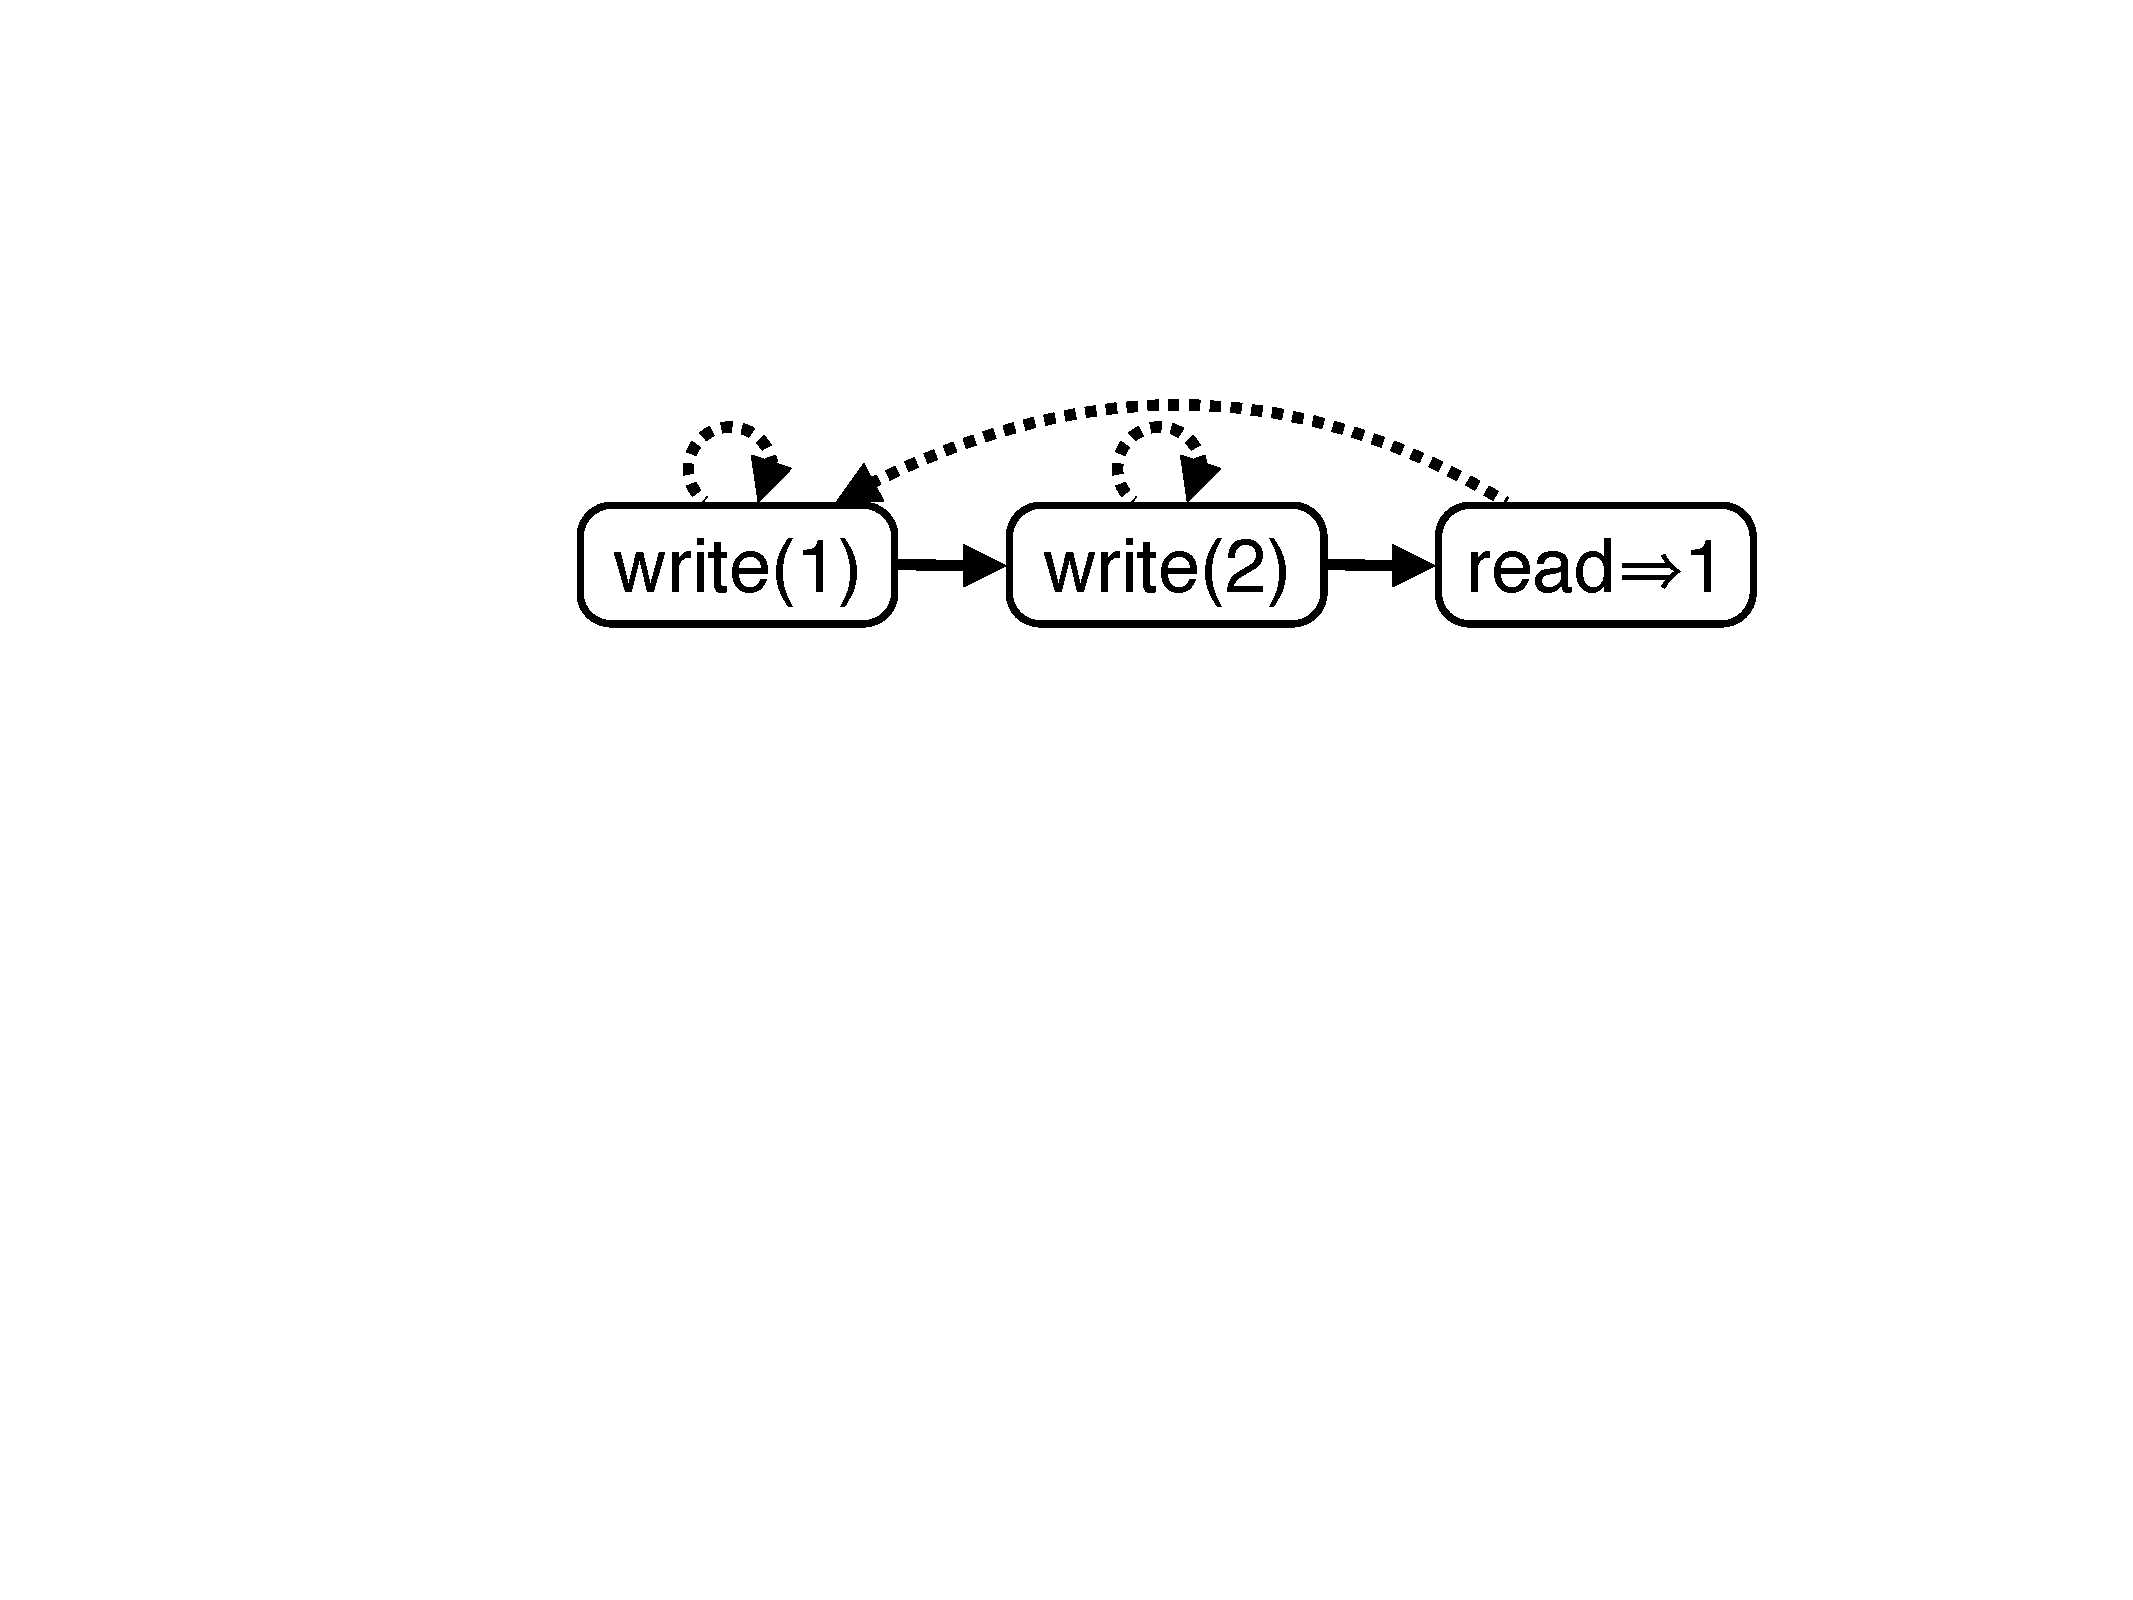
\includegraphics[scale=0.2]{figures/register-pattern-3}
    \caption{Three histories which generate the complement of the atomic
      register ADT kernel.}
    \label{fig:register-patterns}
  \end{figure}

\end{example}
